\documentclass[../candidatura.tex]{subfiles}
\graphicspath{{\subfix{../imagenes/}}}
\begin{document}

\section{Trabajo avanzado}

% en borradores iniciales, la extensión sugerida era de 1 página

\subsection{Prototipado electrónico}

Se ha realizado investigación en nuevas formas de prototipado electrónico, de automatización de procesos de fabricación de electrónica asistida por máquinas, y de documentación de procesos de diseño electrónico. Se han construido los primeros prototipos de fuentes de poder, relojes, secuenciadores, osciladores y amplificadores, y se han puesto a prueba los conceptos y los materiales pedagógicos creados mediante su enseñanza en nuevos cursos de pregrado de diseño de interacción en Chile con un equipo interdisciplinario.

\subsubsection{Chufe y Chufebu: fuente de poder y extensor}

Chufe es un módulo de alimentación para sintetizadores del estándar Eurorack. Tiene como entrada una fuente de poder externa de entre 9V y 15V, con conector tipo barril, y como salida un conector de 16 pines formato Eurorack, con voltajes 12V, -12V, 5V y tierra.

\begin{figure}[htbp]
    \centering
    \includegraphics[width=\textwidth]{./imagenes/chufe/chufe-esquematico.pdf}
    \caption{Esquemático del módulo Chufe}
    \label{fig:chufe-esquematico}
\end{figure}

\begin{figure}[htbp]
    \centering
    \includegraphics[width=0.7\textwidth]{./imagenes/chufe/chufe-placa.pdf}
    \caption{Placa diseñada del módulo Chufe}
    \label{fig:chufe-placa}
\end{figure}

\begin{figure}[htbp]
    \centering
    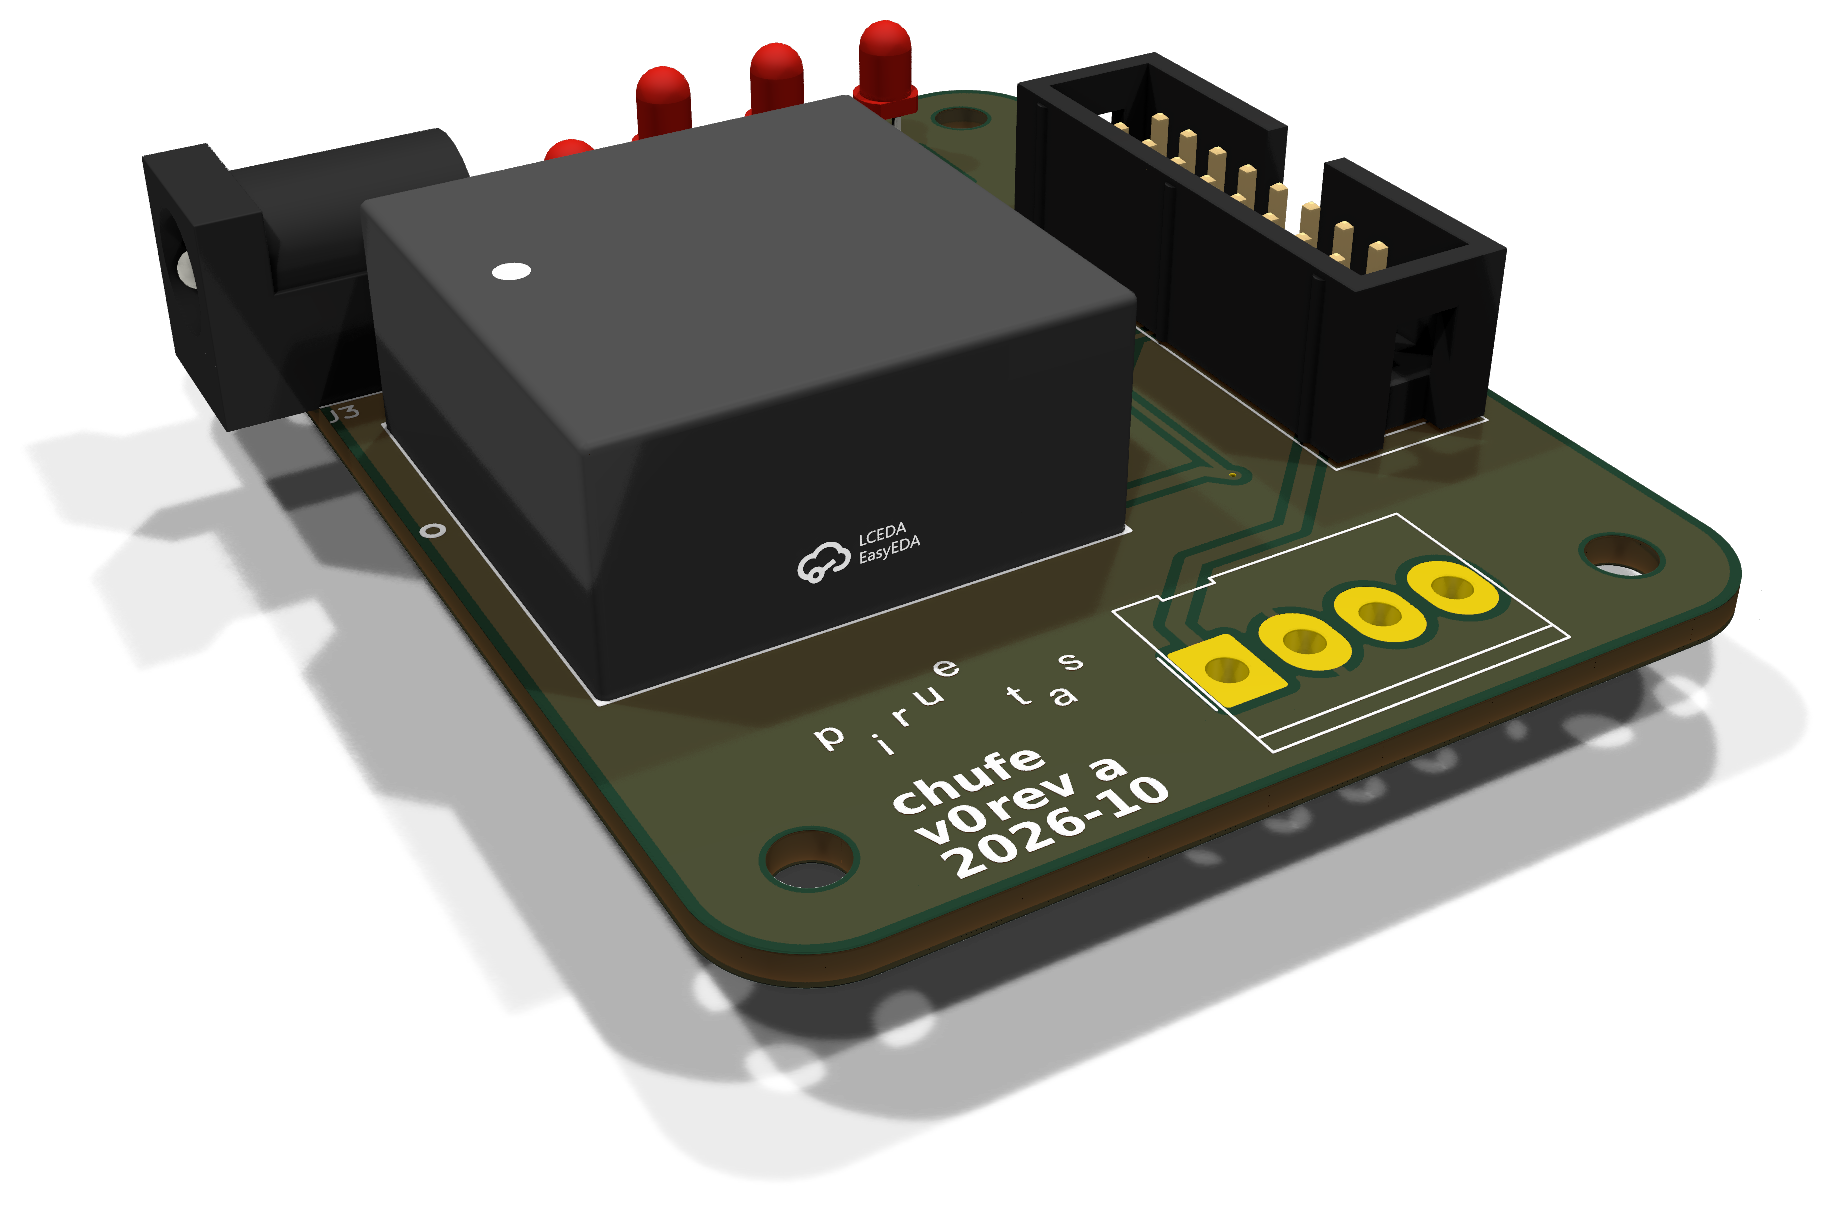
\includegraphics[width=0.7\textwidth]{./imagenes/chufe/chufe-3d-perspectiva.png}
    \caption{Render 3D en perspectiva del módulo Chufe}
    \label{fig:chufe-3d-perspectiva}
\end{figure}

\begin{figure}[htbp]
    \centering
    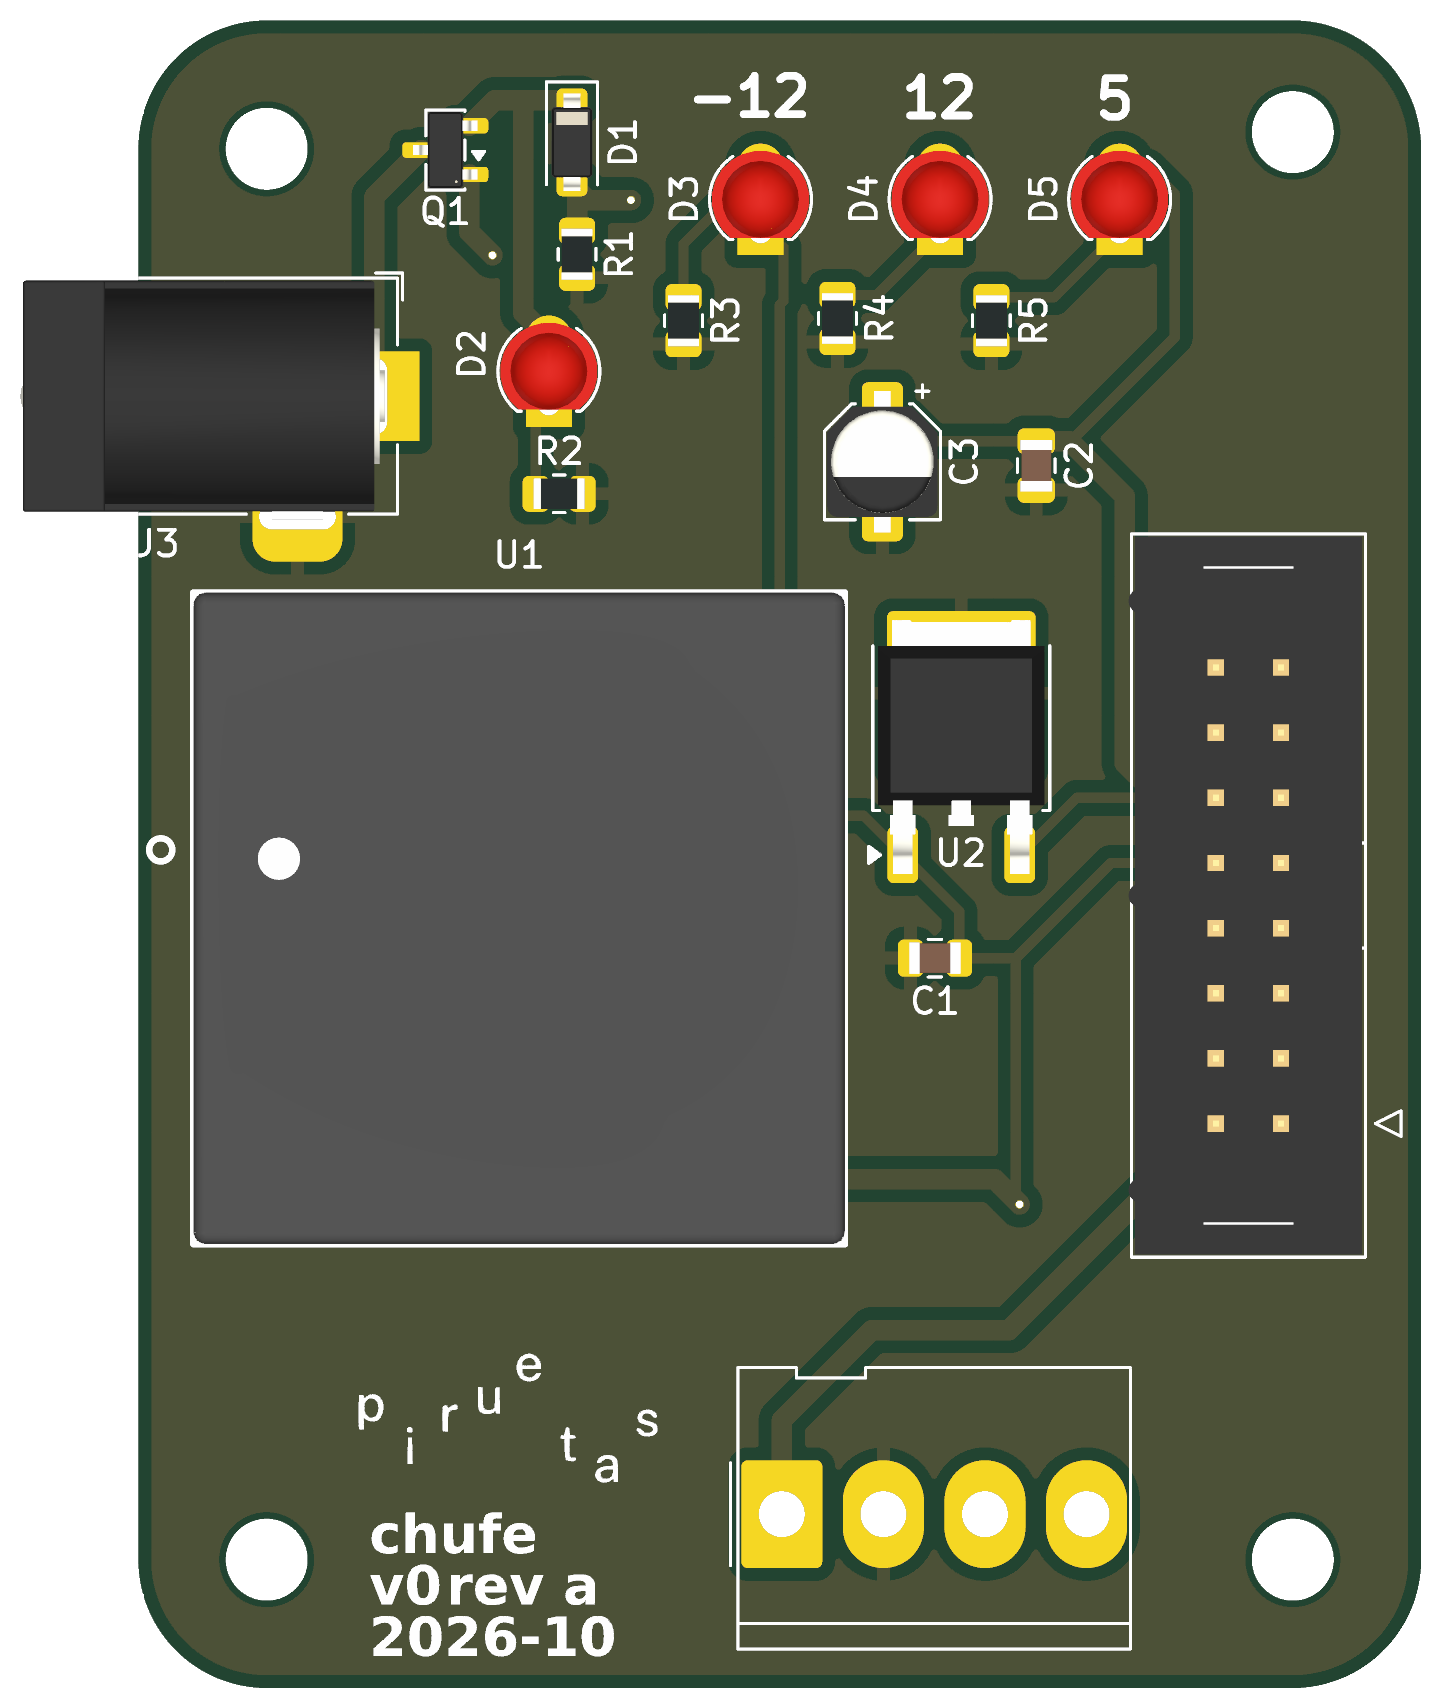
\includegraphics[width=0.4\textwidth]{./imagenes/chufe/chufe-3d-arriba.png}
    \hfill
    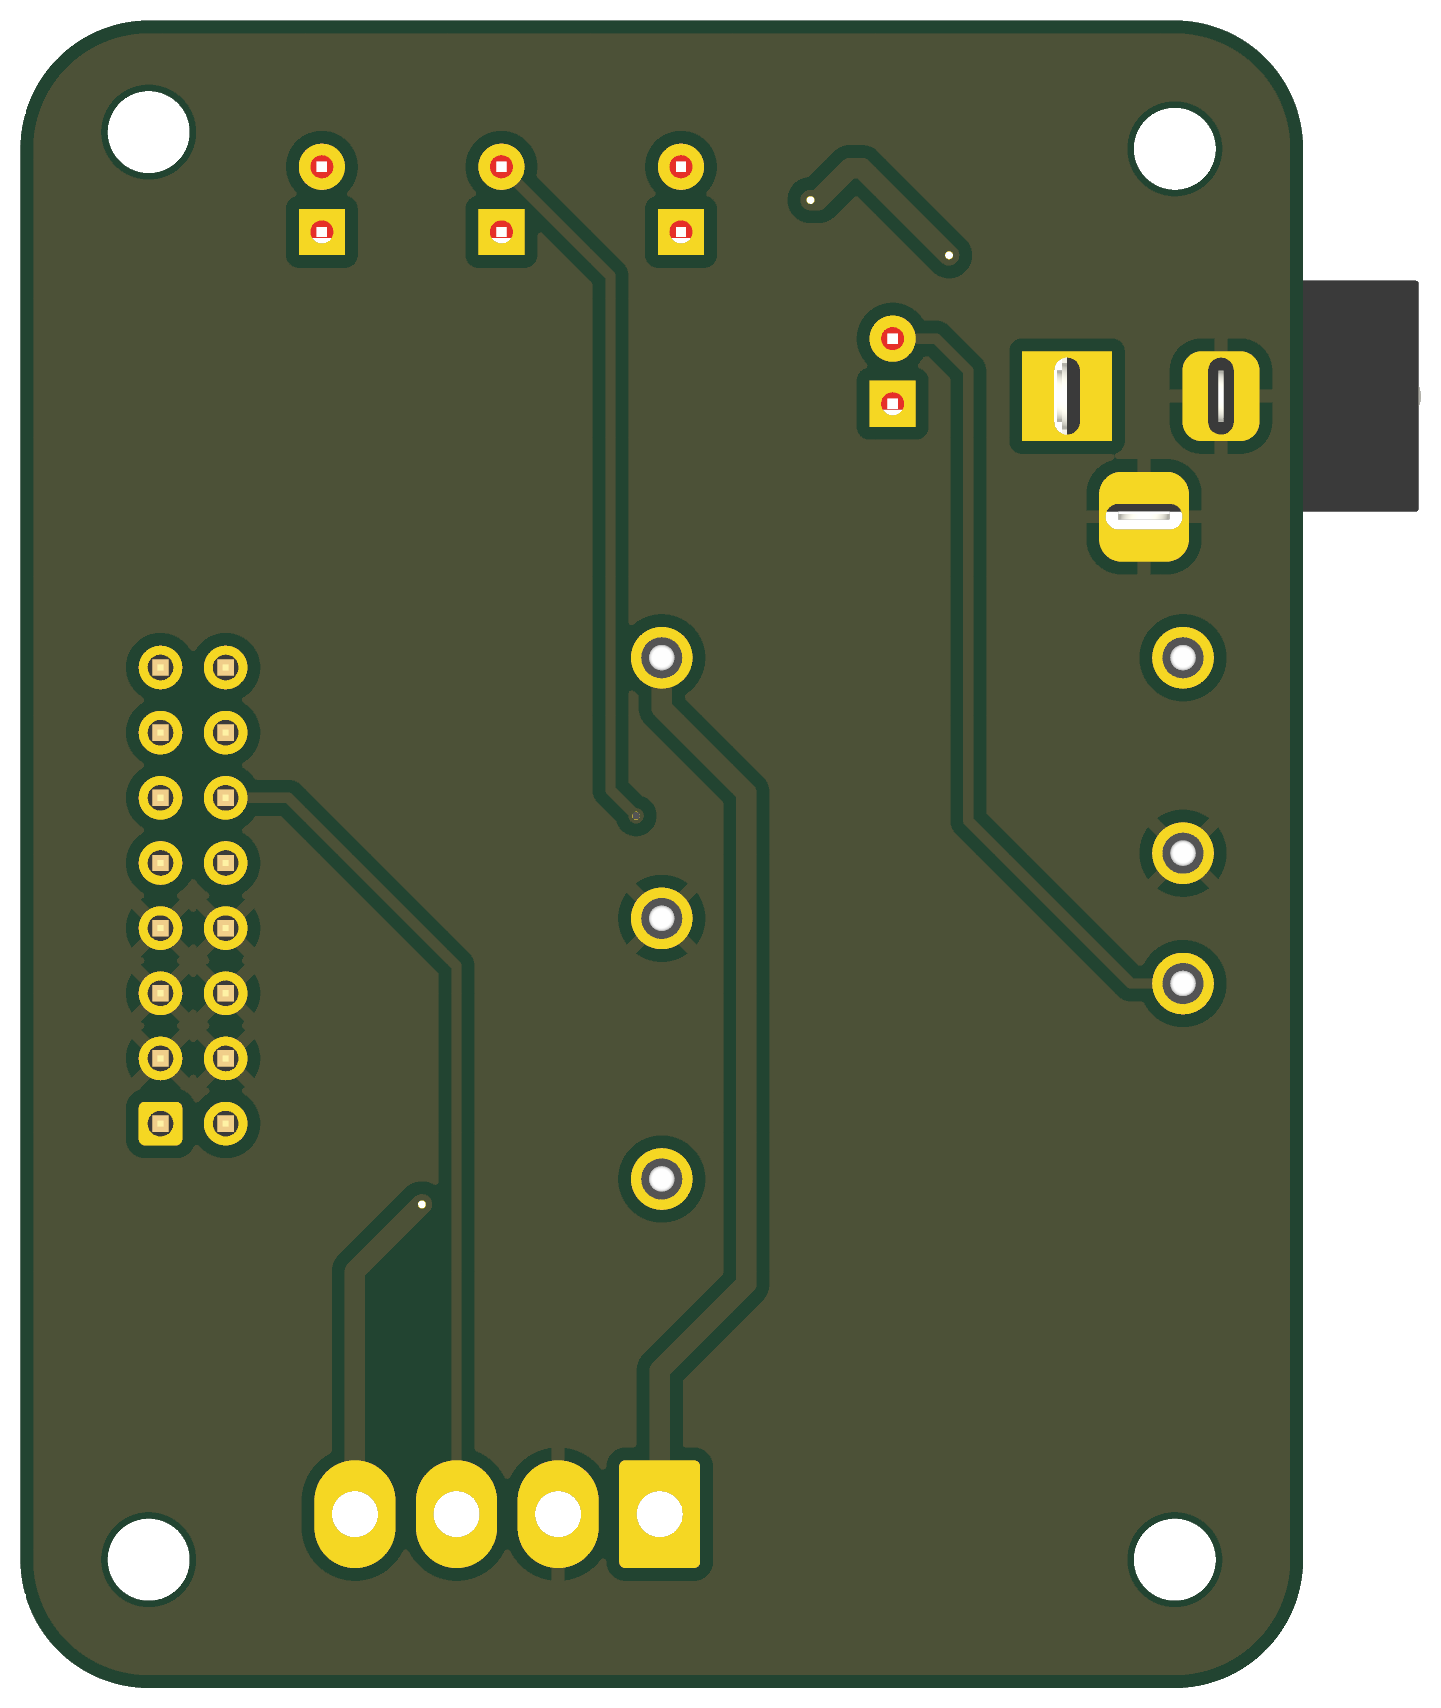
\includegraphics[width=0.4\textwidth]{./imagenes/chufe/chufe-3d-abajo.png}
    \caption{Renders 3D del módulo Chufe, vista superior (izquierda) e inferior (derecha)}
    \label{fig:chufe-3d-arriba-abajo}
\end{figure}

Chufebu es un módulo extensor de Chufe. Tiene como entrada un conector Eurorack de poder, y como salida otros 4 iguales, permitiendo usar un Chufe y poder extenderlo a uno o más buses como Chufebu, según las necesidades del instrumento armado.

Cada uno de estos conectores permite distribuir alimentación a otros módulos de un sistema Eurorack.

Chufebu fue el primero de esta tesis que pasó por el proceso de certificación de la Open Source Hardware Assocation, que fue aprobada en octubre 2026 y se convirtió en mi primer proyecto tanto personal como empresarial en ser certificado, y el décimo de Chile \parencite{piruetas_chufebu_2026}.

\begin{figure}[htbp]
    \centering
    \includegraphics[width=\textwidth]{./imagenes/chufebu/chufebu-esquematico.pdf}
    \caption{Esquemático del módulo Chufebu}
    \label{fig:chufebu-esquematico}
\end{figure}

\begin{figure}[htbp]
    \centering
    \includegraphics[width=0.7\textwidth]{./imagenes/chufebu/chufebu-placa.pdf}
    \caption{Placa diseñada del módulo Chufebu}
    \label{fig:chufebu-placa}
\end{figure}

\begin{figure}[htbp]
    \centering
    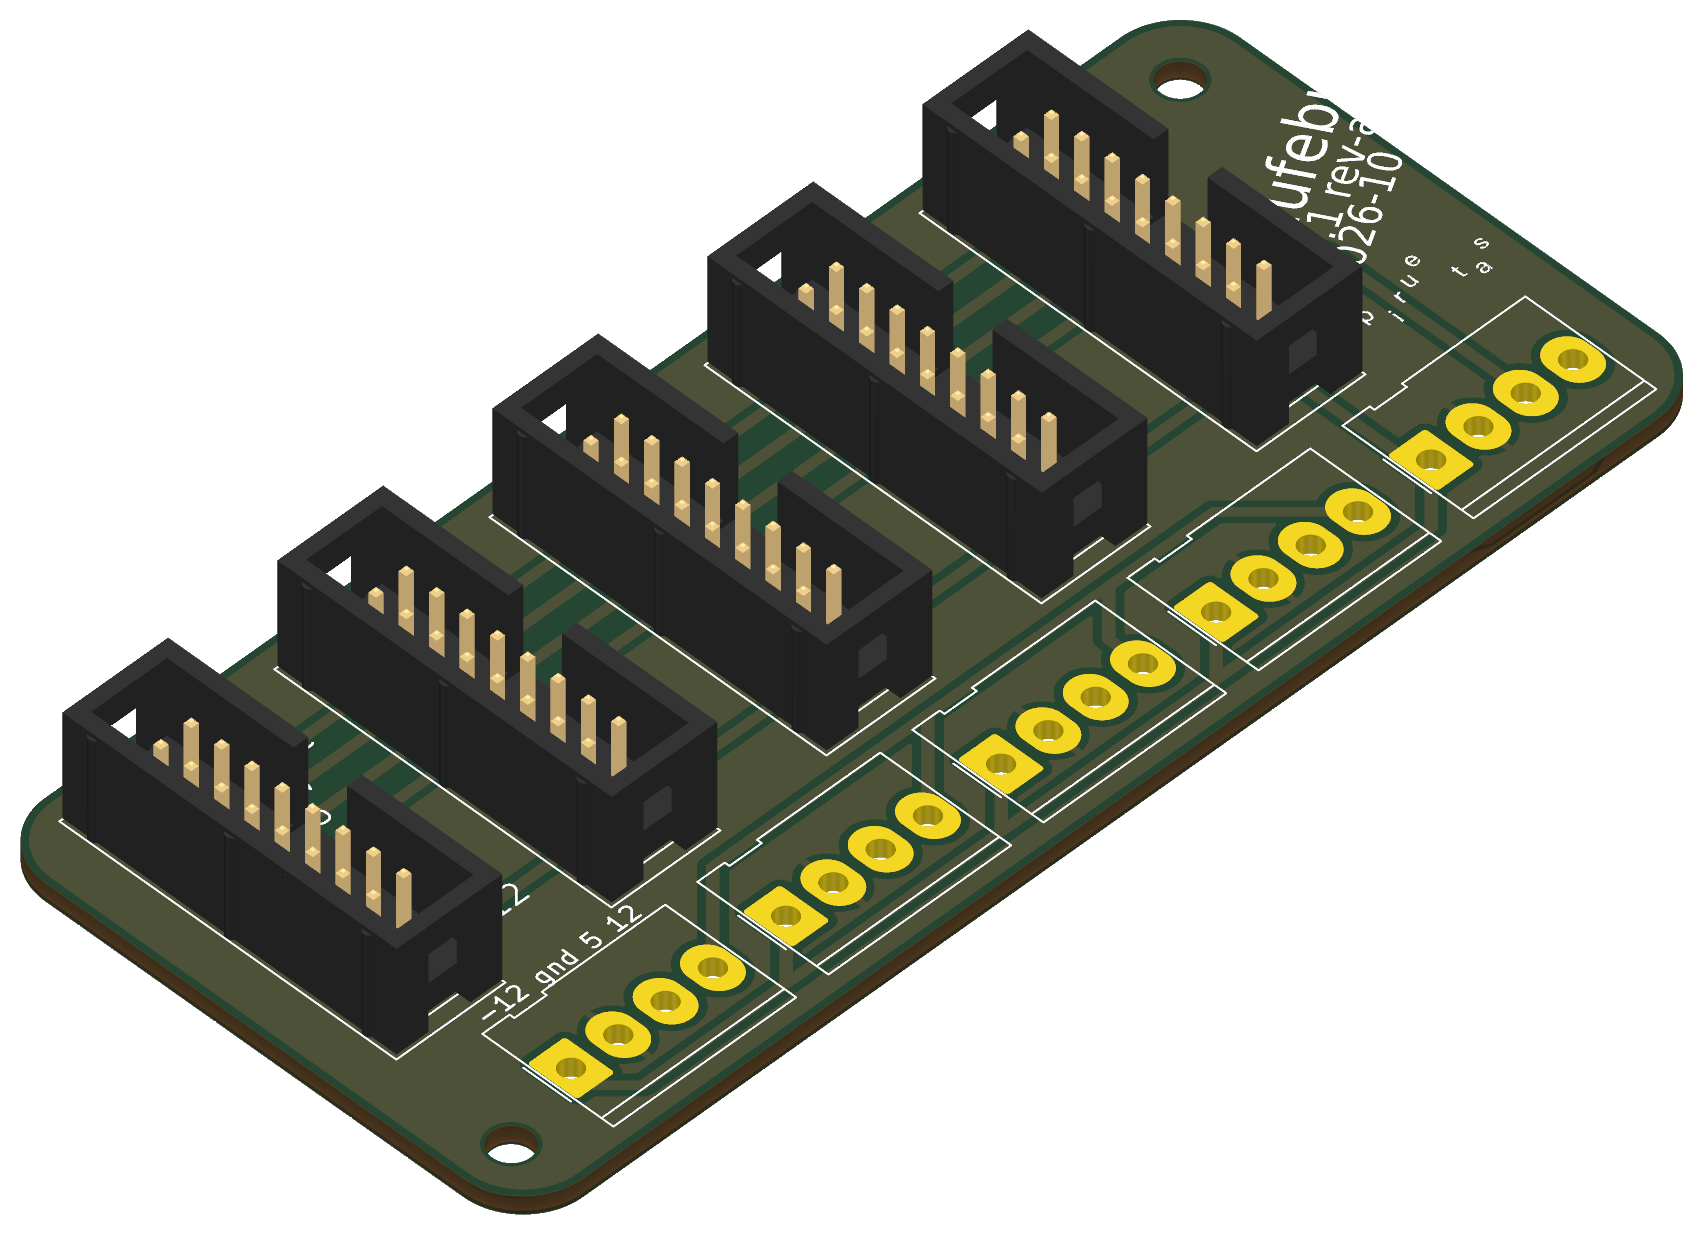
\includegraphics[width=0.7\textwidth]{./imagenes/chufebu/chufebu-3d-iso-frente.png}
    \caption{Render 3D isométrico del módulo Chufebu}
    \label{fig:chufebu-3d-iso-frente}
\end{figure}

\begin{figure}[htbp]
    \centering
    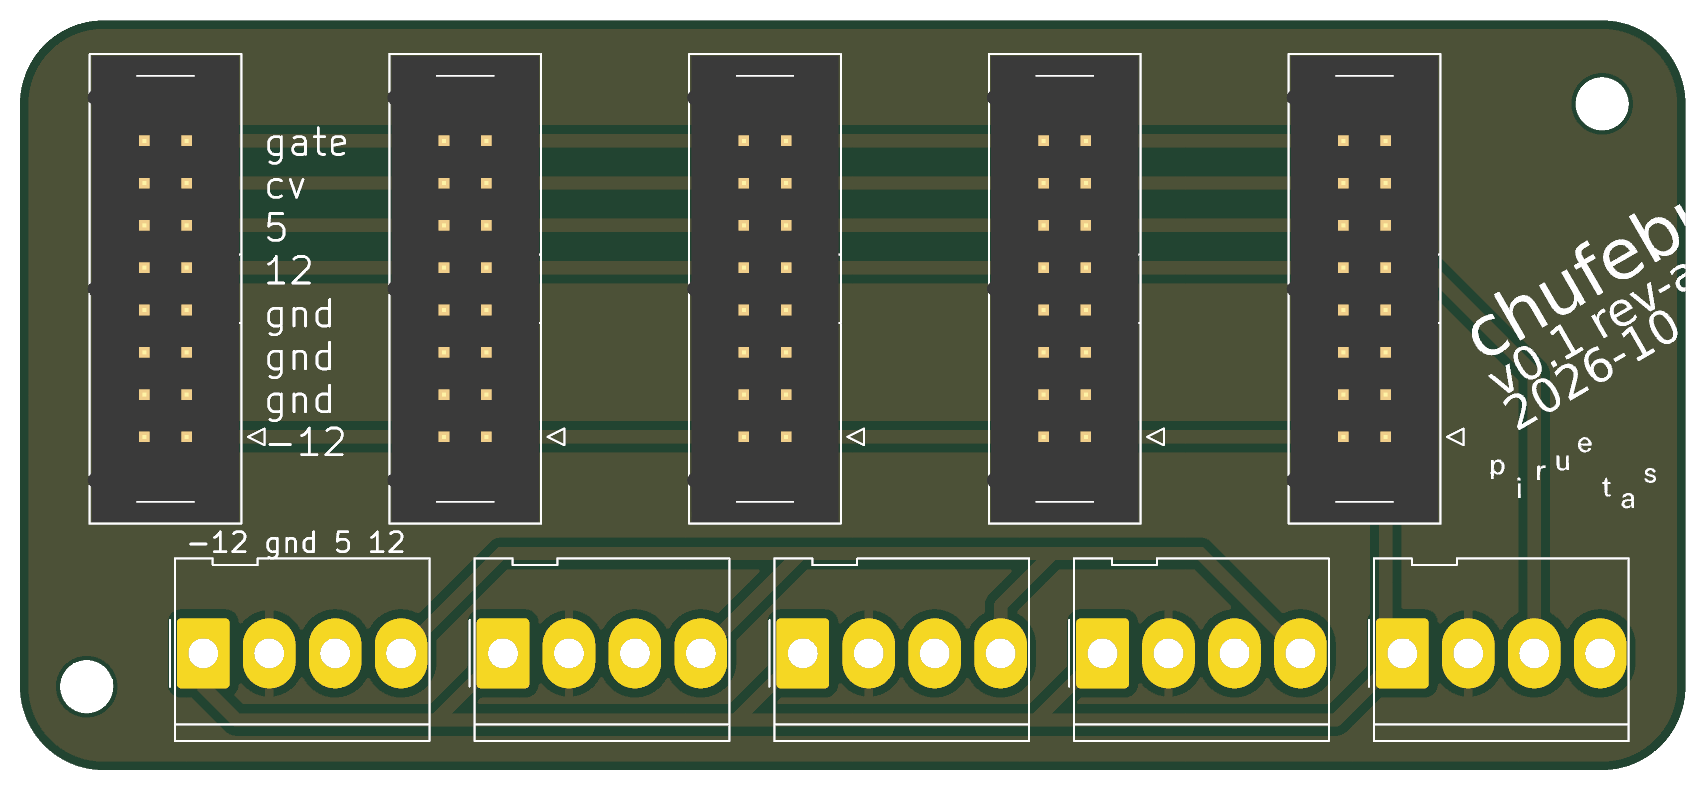
\includegraphics[width=0.8\textwidth]{./imagenes/chufebu/chufebu-3d-arriba.png}

    \vspace{1em}
    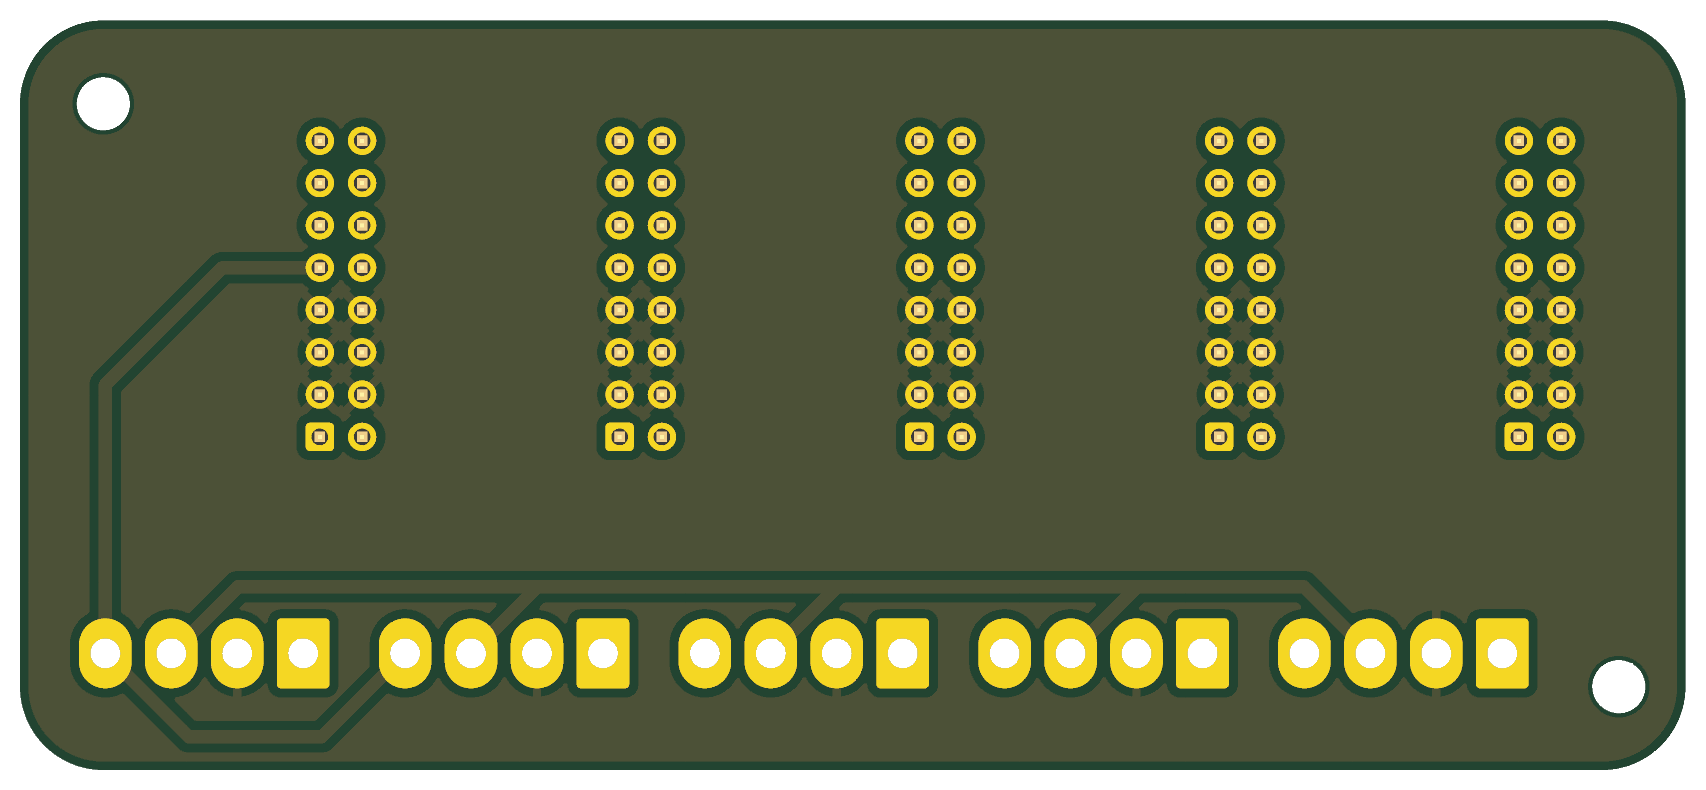
\includegraphics[width=0.8\textwidth]{./imagenes/chufebu/chufebu-3d-abajo.png}
    \caption{Renders 3D del módulo Chufebu, vista superior (arriba) e inferior (abajo)}
    \label{fig:chufebu-3d-arriba-abajo}
\end{figure}


Ambos fueron diseñados usando el software KiCad en octubre de 2026, y su primera revisión está pensada como infraestructura base que permite el desarrollo del resto de esta tesis, y permite desplomar los costos de una fuente de poder Eurorack.

La fuente de poder externa vale 5.000 CLP en un comercio no especializado como MercadoLibre, por eso no se diseña una en esta tesis, y se cuenta con esta base.

Por el otro lado, una fuente de poder Eurorack es un producto nicho, y que tienen muchas barreras de acceso, desde precio, hasta disponibilidad. Una que fue adquirida durante este proceso de diseño y como material de estudio fue el producto Befaco Lunchbus \parencite{befaco_lunchbus_sinfecha}, que tiene un costo del orden de 85 dólares, pero al no tener distribuidor oficial en Chile necesitó de importación y costos adicionales, además del mes que demoró en llegar desde el distribuidor Thonk en Inglaterra.

El precio del orden 80 dólares se condice con las estimaciones supuestas, de que los costos son del orden de 20 dólares en materiales , que necesitan venderlo a su distribuidor al doble para tener ingresos que puedan ser reinvertidos en investigación y desarrollo y que puedan costear el ensamblaje hecho por humanos, y que a su vez distribuidores tienen que vender al orden del doble para pagar su bodegaje y servicios de distribución.

Chufe en su primer prototipo correspondiente a la versión 0.1-rev-a, se fabricaron 5 copias, con un costo de 1.04 USD por placa, más 10.3 USD por placa en materiales soldados de forma automatizada en Hong Kong, para un estimado de 11 USD en la placa.

A esto hay que sumarle envío a Chile 98.78 USD pero repartido entre 100 placas es un estimado de 1 USD por cada placa, más los impuestos pagados de internación por un total de 150.000 CLP, pero también repartidos entre 100 placas para un total de 1.500 CLP por placas.

A grandes rasgos, son 20 USD en Chile por la fuente de poder soldada, en contraste con los 80 USD + envío + impuestos de otra fuente de poder equivalente.

Este precio refleja una construcción de un prototipo funcional, que tras su validación permite pedir grandes cantidades que acceden a descuentos, desplomando aún más el precio.

También se puede tomar la decisión de comercializar estas fuentes de poder a precios acordes a lo popular, dada la naturaleza de la empresa con que se producen estos dispostivos.


\subsection{Prototipado computacional}

Se ha realizado investigación de nuevas formas de automatización computacional, incluyendo la escritura de código y la creación automatizada de documentación, además de estrategias de publicación de bibliotecas de código. Se han ya publicado los primeros prototipos de bibliotecas y herramientas en repositorios públicos.

\subsection{Cursos de electrónica y computación}

En 2024 se crearon en conjunto con el académico y artista Matías Serrano una serie de cursos de pregrado que dictamos en la Escuela de Diseño de la Universidad Diego Portales: el primer semestre dictamos "DIS8644 Taller de diseño de máquinas electrónicas", y en el segundo semestre "DIS8645 Taller de diseño de máquinas computacionales".

La primera versión de cada curso la dictamos en el año 2025, y la segunda este 2026, con la métrica de que son los talleres de tercer y cuarto año de diseño con mayor lista de espera y cantidad de estudiantes inscritos en la Escuela de Diseño de la Universidad Diego Portales.

Como parte de nuestras investigaciones doctorales y prácticas conjuntas, empezamos este 2026 a escribir un libro académico de pregrado titulado "Máquinas sonoras", que esperamos sirva de antesala a nuestras tesis doctorales individuales, y que se convierta en un texto de referencia para cursos de enseñanza de sonido, electrónica y programación como los que dictamos.

También desde 2026 se empezó a dictar \textit{DIS09214 Pensamiento computacional}, un nuevo curso obligatorio para segundo año de diseño, enfocado en los fundamentos de la computación aplicados a la creación de gráficas interactivas con la herramienta p5.js. Se están sistematizando y ampliando los apuntes del curso para su publicación como libro académico, con la esperanza de que se convierta en un aporte significativo en diseño, artes y disciplinas afines.

\subsection{Infraestructura comercial}

A nivel individual se ha realizado la infraestructura comercial y técnica, incluyendo la constitución de una empresa, Piruetas SpA, que permite financiar la investigación y desarrollo de los productos asociados a esta tesis doctoral, además de la contratación de personal, pasantes académicos y practicantes profesionales, desde el año 2022 hasta la fecha.

\end{document}